%%RESULTADOS

\section{Adquisición de datos}
Tras adquirir las señales patrón para la evaluación del bloque de adquisición descritas en la metodología, se calculó la métrica de correlación entre las señales adquiridas y las patrón, buscando traslapar una sobre otra como se muestra en la Figura \ref{Figura: ValProCum}.
Al tener el valor de correlación para cada registro se obtuvo como resultado una correlación promedio de 0.9615 $\pm$ 0.0604, valor que sirve como indicador de la calidad del bloque diseñado para la adquisición y decodificación de datos.

\begin{figure}[htbp]
	\centering
	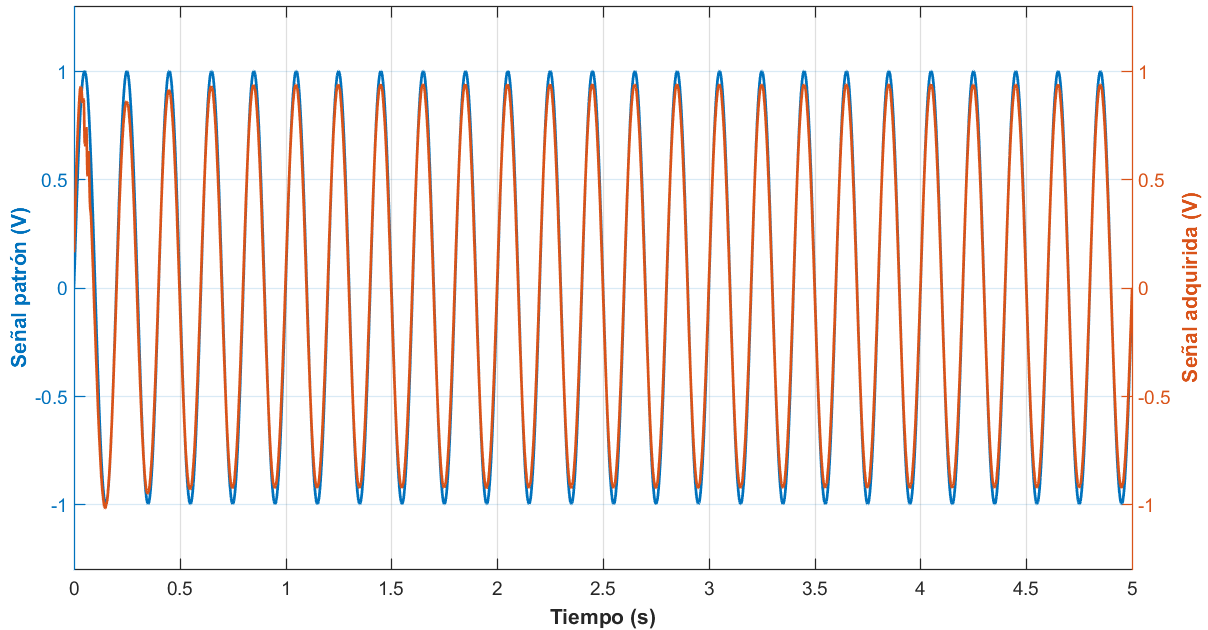
\includegraphics[width=\textwidth]{ValProCum.png}
	\caption{Comparación entre señal adquirida con el bloque de adquisición diseñado (rojo) y señal patrón (azul)}
	\label{Figura: ValProCum}
\end{figure}


\section{Procesamiento de sEMG}
Utilizando los registros de calibración se probaron los filtros diseñados, obteniendo como resultado notorio la estabilización de la línea base de cada registro. En la Figura \ref{Figura: Filtrado} se muestra una comparación entre los registros crudos y filtrados de ambos canales adquiridos durante el entrenamiento.

\begin{figure}[htbp]
	\centering
	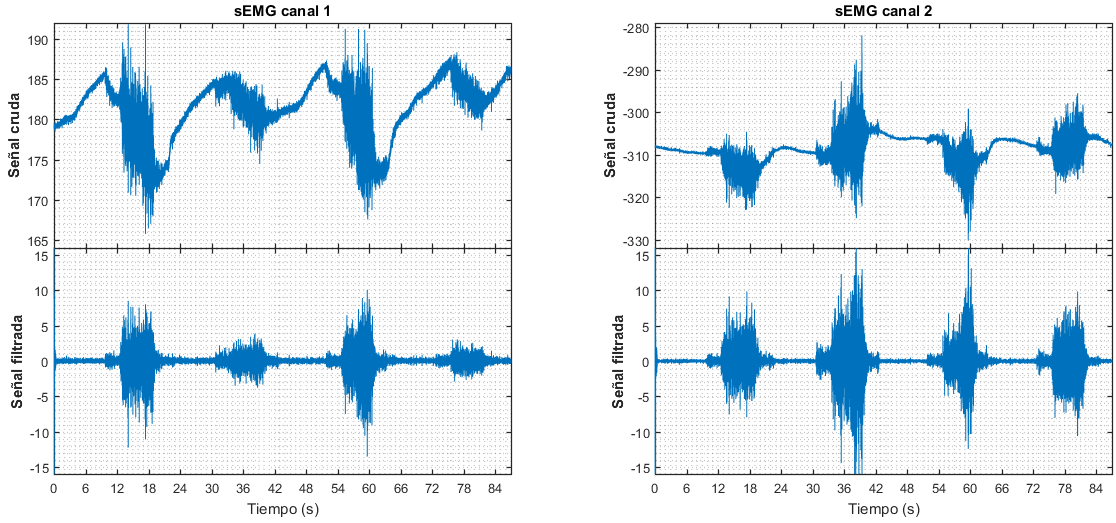
\includegraphics[width=\textwidth]{Filtrado.png}
	\caption{Ejemplo representativo del funcionamiento de los filtros diseñados aplicados a registros de entrenamiento.}
	\label{Figura: Filtrado}
\end{figure}

Con los registros ya filtrados se obtuvo el valor RMS a lo largo de todo el registro utilizando ventanas de 100 ms, dando como resultado una envolvente discreta de sEMG para cada canal. En la Figura \ref{Figura: RMS} se muestran los registros de sEMG filtrados con sus respectivas envolventes discretas de RMS y marcadores de la acción solicitada al sujeto durante el entrenamiento.

\begin{figure}[htbp]
	\centering
	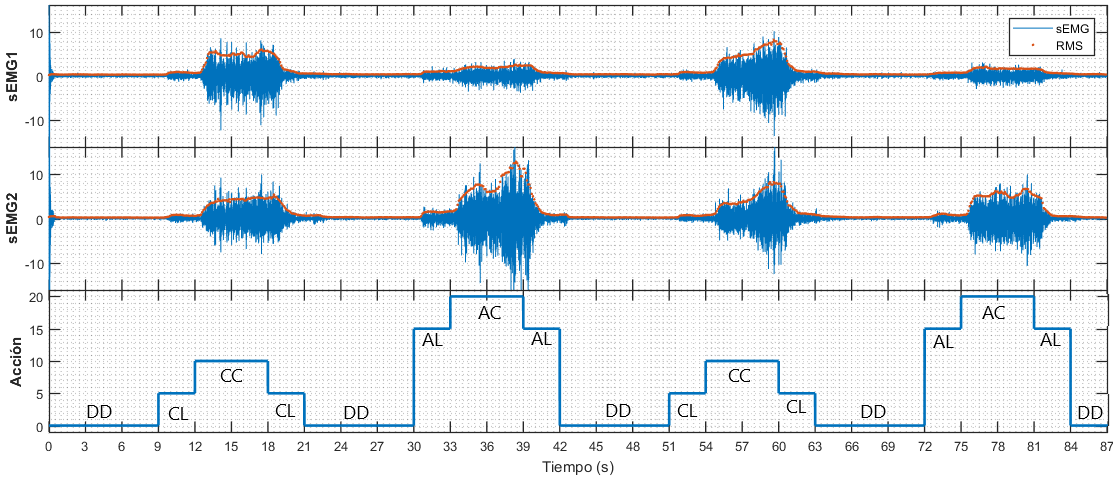
\includegraphics[width=\textwidth]{RMS_m.png}
	\caption{Ejemplo representativo de la obtención de envolvente discreta de RMS en registros de entrenamiento. Arriba: Canal 1 de sEMG. Medio: Canal 2 de sEMG. Abajo: Marcadores de acción solicitada al sujeto (descanso (DD), cierre ligero (CL), cierre completo (CC), apertura ligera (AL), apertura completa (AC)). Las envolventes (puntos rojoss) fueron multiplicadas por 2 para fines de visualización.}
	\label{Figura: RMS}
\end{figure}

\section{Esquema de control}
Previo a realizar pruebas del esquema de control en línea, este se probó fuera de línea, aprovechando los registros de calibración. Para estas pruebas se diseñó un script en MATLAB que obtiene los parámetros necesarios del esquema de control de la misma forma que los arroja la calibración. Una vez obtenidos dichos parámetros se configura con ellos al esquema de control y se realiza una prueba fuera de línea donde con cada ventana de sEMG se obtiene un valor de RMS el cuál es sometido al esquema de control y arroja un valor de amplitud para el canal asociado al movimiento detectado. Tras probar el esquema de control con tres registros distintos de calibración se obtuvo un porcentaje de acierto del 81$\%$ en la identificación correcta de los movimientos de cierre, apertura y descanso de mano.

En la Figura \ref{Figura: MapOff} se muestra el resultado de  una prueba exitosa del esquema de control fuera de línea, donde se observa que el esquema de control diseñado suele presentar errores en la identificación de los segmentos iniciales y finales de la tarea apertura de mano.

\begin{figure}[htbp]
	\centering
	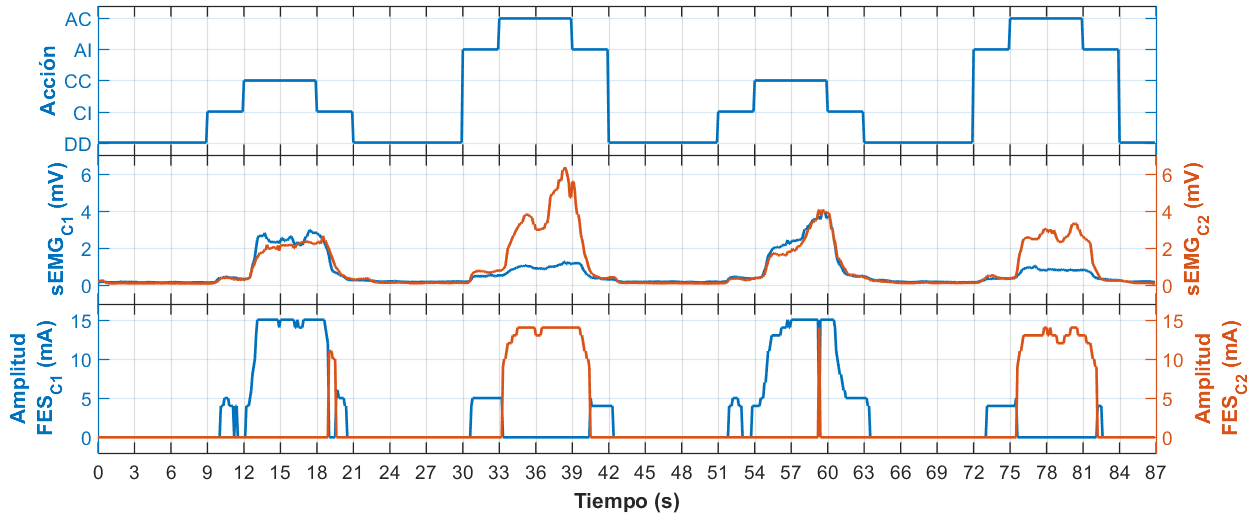
\includegraphics[width=\textwidth]{MapOff.png}
	\caption{Ejemplo exitoso representativo de las pruebas del esquema de control funcionando fuera de línea con registros de calibración. Arriba: Envolventes de sEMG (Azul: canal 1. Rojo: canal 2). Medio: Amplitudes de estimulación resultantes del sistema de control (Azul: canal 1. Rojo: canal 2). Abajo: Marcadores de acción solicitada al sujeto (descanso (DD), cierre ligero (CL), cierre completo (CC), apertura ligera (AL), apertura completa (AC)).}
	\label{Figura: MapOff}
\end{figure}

\newpage
Para la prueba en línea se configuró el modelo de Simulink con los datos obtenidos tras la calibración, y se solicitó al sujeto realizar el seguimiento de un par de señales trapezoidales que le indicarían el tipo de movimiento que tendría que lograr. Cuando la trapezoidal estuviera en cero, tendría que mantenerse en descanso; en la pendiente positiva de la trapezoidal tendría que realizar una transición de descanso hacia el movimiento completo solicitado; en la meseta de la trapezoidal tendría que mantener el movimiento completo solicitado; y en la pendiente negativa de la trapezoidal tendría que realizar una transición del movimiento completo solicitado hacia descanso.

En la Figura \ref{Figura: MapOn} se muestra un segmento de una de las pruebas exitosas realizadas en línea. En dicha figura se puede observar que existe un retardo entre la trapezoidal y la respuesta del sistema de control, el cual es la suma del retardo que genera el procesamiento de la señal, el retardo ocasionado por el esquema de control, y el tiempo de respuesta del sujeto a la indicación de la trapezoidal.

\begin{figure}[htbp]
	\centering
	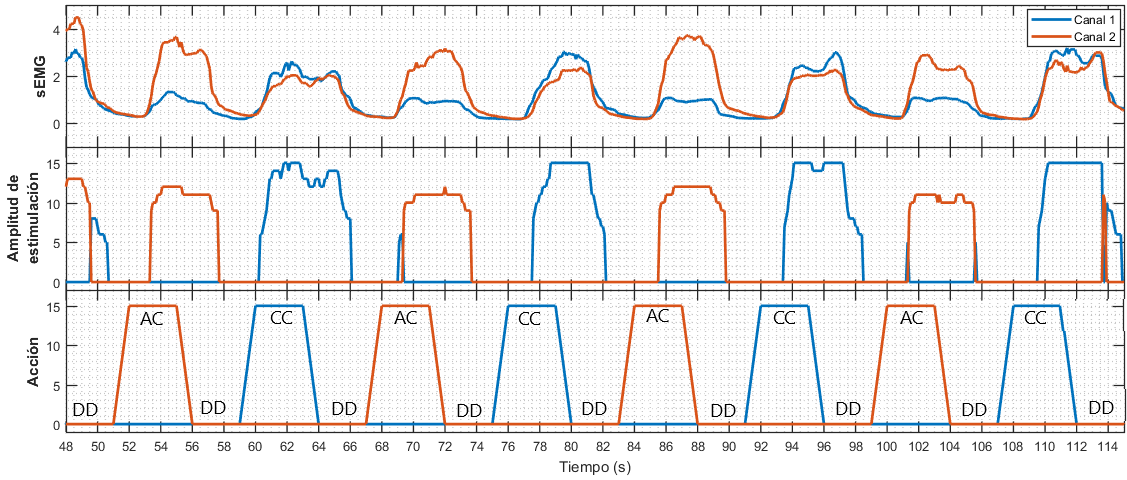
\includegraphics[width=\textwidth]{MapOn.png}
	\caption{Ejemplo exitoso representativo de las pruebas del esquema de control funcionando en línea. Arriba: Envolventes de sEMG (Azul: canal 1. Rojo: canal 2). Medio: Amplitudes de estimulación resultantes del sistema de control (Azul: canal 1. Rojo: canal 2). Abajo: Señales indicadoras de tarea a seguir (descanso (DD), apertura de mano (AC), cierre de mano (CC)).}
	\label{Figura: MapOn}
\end{figure}

Para obtener el valor del retardo total se midió el tiempo existente entre el inicio de la pendiente positiva de la señal indicadora (trapezoidal) y la activación de la estimulación eléctrica. Al promediar los tiempos obtenidos a lo largo de las pruebas realizadas en línea se obtuvo un valor de 2.3 $\pm$ 0.3553 s.

En la Figura \ref{Figura: Retardo} se muestra un acercamiento a las señales obtenidas en una prueba representativa de las pruebas realizadas en línea. Se muestran una sobre otra para visualizar el retardo existente entre el inicio de la señal indicadora y la activación de la estimulación eléctrica.

\begin{figure}[htbp]
	\centering
	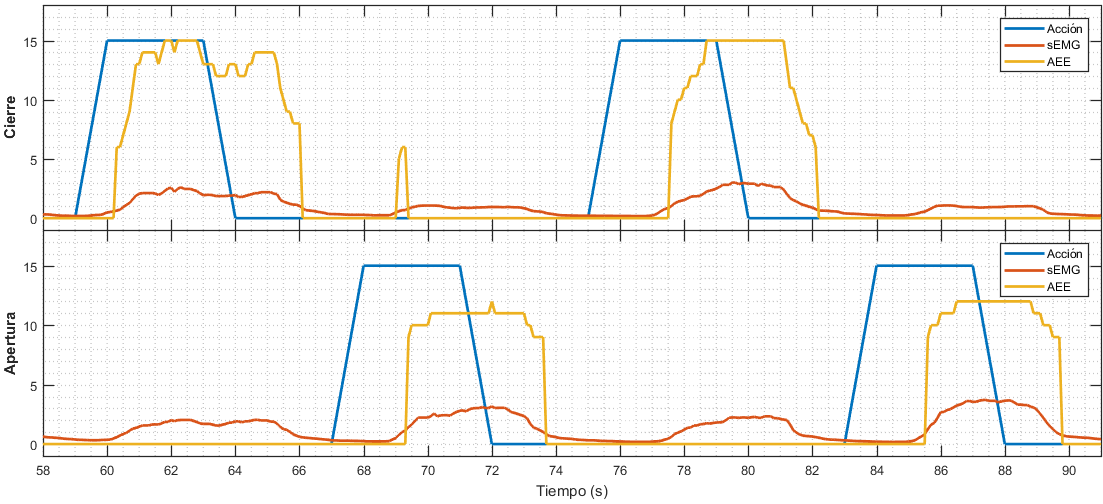
\includegraphics[width=\textwidth]{Retardo.png}
	\caption{Acercamiento a prueba representativa de las pruebas del esquema de control funcionando en línea. Se muestran las diferentes señales asociadas a cada movimiento una sobre otra para visualizar el retardo existente. Arriba: Señales para movimiento cierre de mano. Abajo: Señales para movimiento apertura de mano. En azul se muestra la señal indicadora del movimiento a realizar. En rojo se muestra la envolvente de sEMG. En amarillo se muestra la amplitud de estimulación eléctrica (AEE) arrojada por el esquema de control.}
	\label{Figura: Retardo}
\end{figure}





